\chapter{Uživatelský interface}
Komunikaci testlabu s~jeho uživateli obsluhuje webová aplikace. Webová aplikace je vytvořena pomocí technologií html, css, php a~javascript. Pomocí webové aplikaci bude možné prohlížet modely všech zařízení a~jednotlivé modely upravovat. Model zařízení obsahuje všechny informace o testovaném zařízení, například IP adresu zařízení, informace o vložené SIM kartě a~podporované funkce. V~neposlední řadě je možné zjistit informace o všech vykonaných testech zařízení a~překladech firmwarů. Jednotlivé možnosti zobrazení a~úpravy informací jsou popásány v~následujících sekcích.

\section{Sekce build}
Sekce build zobrazuje všechny informace o stahování zdrojových kódů z repozitářů a~jejich následné kompilaci. Sekce je prozatím rozdělena na~tři stránky list release, build platforms a~build products. První stránka zobrazuje informace o jednotlivých releasech a~ve zbylých dvou stránkách nalezneme informace o překladech všech firmwarů.

\subsection{Stránka List releases}
První stránka list releases sekce build informuje o všech vytvořených verzích. Release je vytvořen při každém spuštění programu testlab a~jsou k němu vázány všechny informace celého průběhu testování. Stránka obsahuje pouze jednu tabulku, kde každý řádek odpovídá jednomu vytvořenému releasu.

\begin{figure}[h]
  \centering
  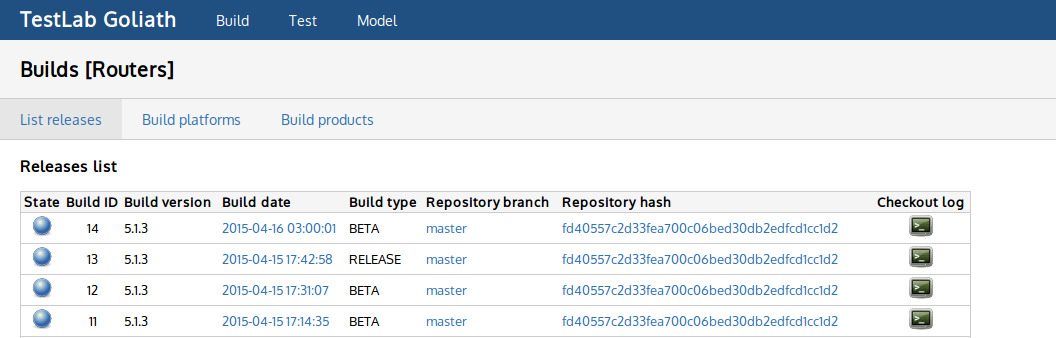
\includegraphics[width=\LW]{web_build_release}
  \caption{Stránka release sekce build}
  \label{fig:web_build_release}
\end{figure}

Tabulka má celkem osm sloupců. První sloupec state informuje o výsledku stažení nebo~aktualizaci zdrojových kódu testovaného projektu. Sloupec state rozlišuje dva stavy jimiž jsou modrá kulička při úspěšném stažení zdrojových kódů a~červená kulička při neúspěšném stažení zdrojových kódů. Sloupec Build ID zobrazuje jedinečné číslo identifikující každý release, které musí být v~jednom projektu u každého releasu unikátní. Sloupec build version zobrazuje verzi překládaných zdrojových kódů. Build date zobrazuje datum a~čas, kdy bylo testování spuštěno. Sloupec build type informuje, zdali testovaný release byl ve fázi BETA nebo~ve fázi ostrého releasu určeného pro zákazníky. Sloupec repository branch informuje, z jaké větve repositáře byl firmware překládán a~sloupec repository hash zobrazuje hash posledního commitu testovaného zdrojového kódu. V~posledním sloupci je umístěn odkaz na~log z průběhu stahování či~aktualizace zdrojových kódů testovaného releasu.

\subsection{Stránka Build platforms}
Builds platform je přehledová stránka zobrazující výsledky překladů testovaných platforem. Aktuální zobrazovaný release je zobrazen v~nadpisu této stránky. Dále stránka build platforms obsahuje dvě tabulky. První dominantní tabulka zobrazuje výsledky překladů a~obsahuje pouze dva sloupce. První sloupec state zobrazuje výsledek překladu platformy a~druhý sloupec platform obsahuje názvy překládaných platforem. Název platformy slouží také jako odkaz na~přehled překladů všech výrobků této platformy. Druhá menší tabulka obsahuje pouze jeden sloupec se seznamem odkazů na~překlady platforem posledních releasů.

\begin{figure}[h]
  \centering
  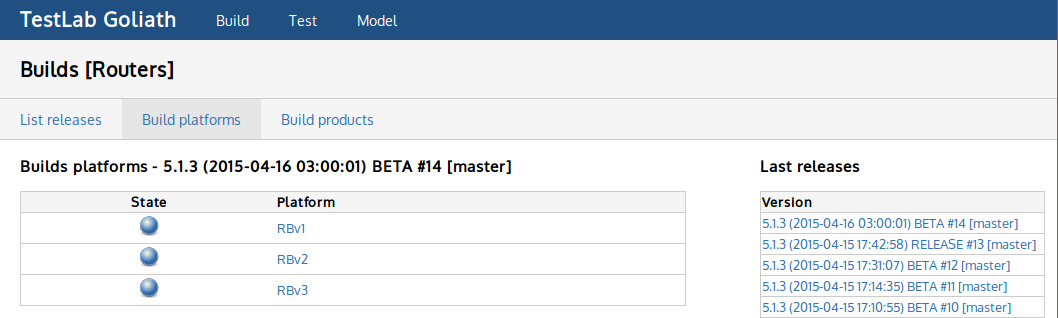
\includegraphics[width=\LW]{web_build_platform}
  \caption{Stránka platform sekce build}
  \label{fig:web_build_platform}
\end{figure}

\subsection{Stránka Build products}
Stránka build products již zobrazuje konkrétní informace o překladu vybraných produktů. Stránka má totožné rozložení s~předchozí stránkou build platforms. Zde první tabulka informuje o překladech produktů a~obsahuje celkem pět sloupců. První sloupec state indikuje výsledek překladu firmwaru. Sloupec product obsahuje název firmwaru překládaného produktu. Sloupec platform zobrazuje platformu daného produktu. V~případě úspěšného přeložení firmwaru jsou ve sloupci firmware odkazy na~soubory s~přeloženým firmwarem. Poslední sloupec logs obsahuje odkazy na~logy z každého překladu, pomocí nichž lze jednoduše hledat případné chyby při překladu. Druhá tabulka má totožný obsah i význam jako u předchozí stránky build platforms.

\begin{figure}[h]
  \centering
  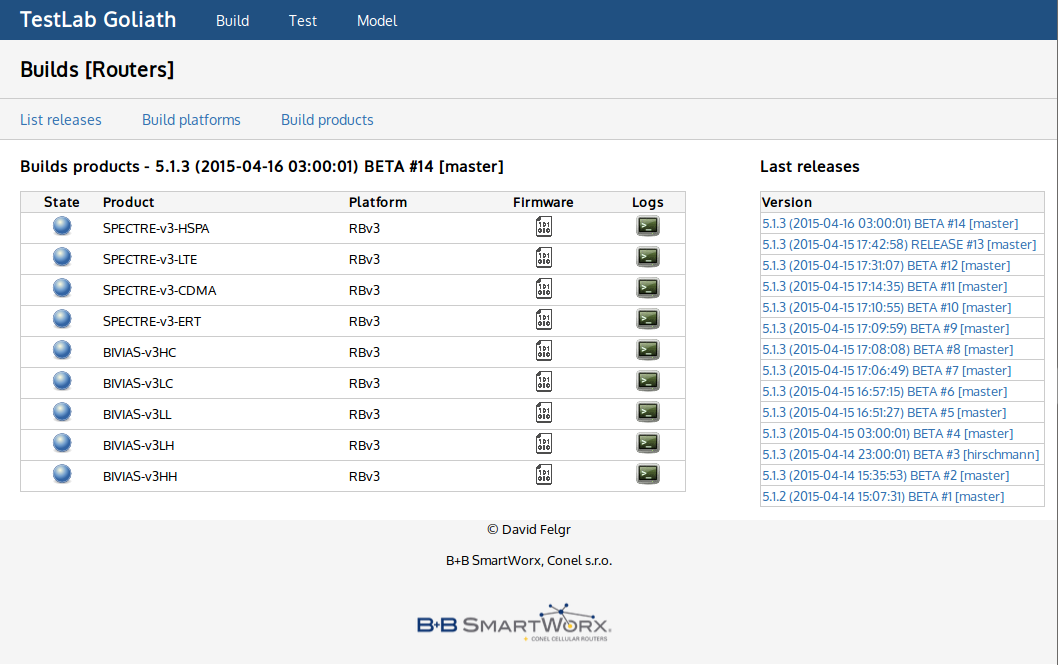
\includegraphics[width=\LW]{web_build_product}
  \caption{Stránka product sekce build}
  \label{fig:web_build_platform}
\end{figure}

\section{Sekce test}
Sekce test shromažďuje všechny informace z druhé fáze testování, kdy je přeložený firmware nahrán do jednotlivých zařízení, a~ty jsou následně testovány. Sekce test obsahuje celkem čtyři stránky. První stránka devices zobrazuje přehled testování jednotlivých zařízení v~každé verzi firmwaru. Stránka functions zobrazuje přehled testování funkcí na~jednotlivých zařízeních. Stránka procedure zobrazuje výsledky zvolených testovacích procedur na~jednotlivých zařízeních. Poslední stránka log vypisuje chybové hlášky vzniklé při průběhu testování.

\subsection{Stránka Devices}
První stránka devices sekce test obsahuje pouze jednu tabulku. V~jednotlivých sloupcích tabulky jsou všechna testovaná zařízení a~každý řádek obsahuje informace o jedné testované verzi firmwaru. Každá buňka uvnitř tabulky zobrazuje informaci a~výsledku průběhu testů na~zařízení v~určité verzi firmwaru. Výsledek testů může být buď úspěšný, což signalizuje zelená fajfka, nebo~může být neúspěšný, což signalizuje červený křížek. Červený křížek také slouží jako odkaz na~logy neúspěšných testů odpovídajícího zařízení. V~případě že, zařízení nebylo testováno, zůstává buňka prázdná.

\begin{figure}[h]
  \centering
  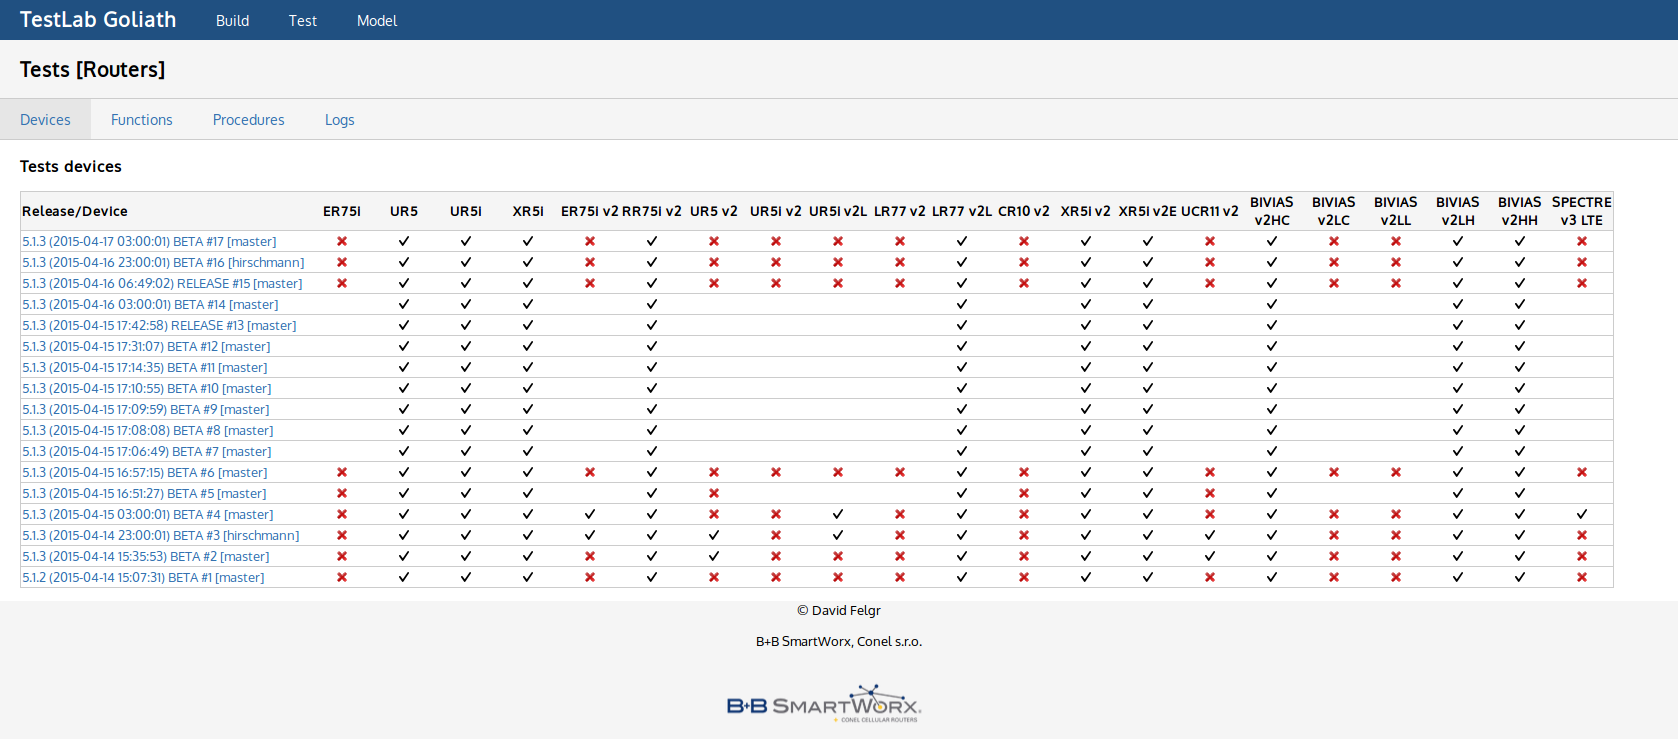
\includegraphics[width=\LW]{web_test_device}
  \caption{Stránka product sekce build}
  \label{fig:web_test_device}
\end{figure}

\subsection{Stránka Functions}
Stránka functions slouží k zobrazení přehledu testů jedné testované verze firmwaru. Verzi firmwaru je možné si vybrat pomocí pravé tabulky obdobně jako na~stránce builds platform nebo~přechodem z předchozí stránky devices. Informace o aktuálním zobrazeném releasu jsou umístěny v~nadpisu stránky. V~hlavní tabulce jsou zobrazeny výsledky testů funkcí na~jednotlivých zařízeních. Každý sloupec představuje jedno zařízení, každý řádek představuje jednu funkci a~všechny buňky uvnitř tabulky zobrazují výsledek testu funkce na~daném routeru. Ikona zobrazující neúspěšný test je zároveň odkaz na~výpis logu neúspěšných procedur odpovídající funkce.

\begin{figure}[h]
  \centering
  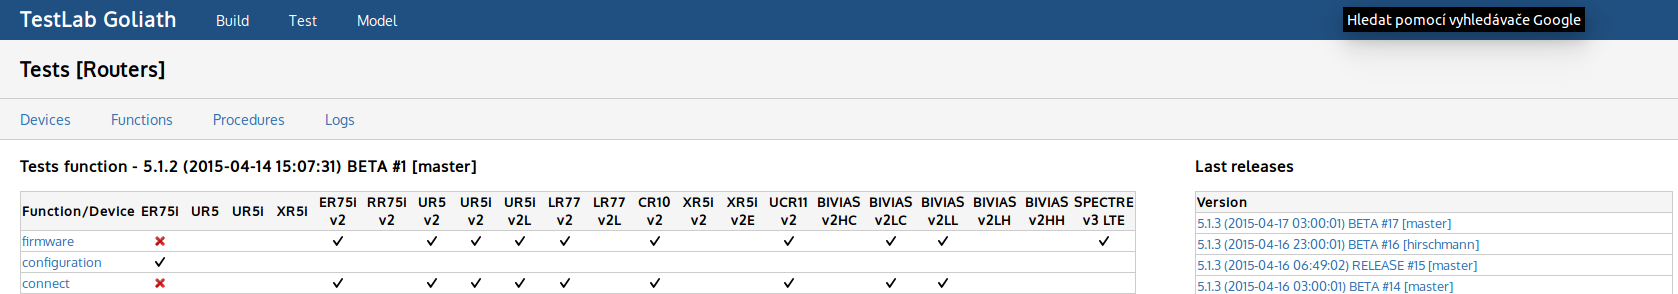
\includegraphics[width=\LW]{web_test_function}
  \caption{Stránka product sekce build}
  \label{fig:web_test_device}
\end{figure}

\subsection{Stránka Procedures}
Stránka procedures zobrazuje výsledky všech spuštěných testovacích procedur nebo~pouze výsledky testovacích procedur jedné vybrané funkce. Funkci si lze vybrat na~předchozí stránce functions. Rozložení a~funkce stránky jsou zcela totožné se stránkou functions, pouze místo funkcí jsou zobrazovány již konkrétní testovací procedury a~jejich výsledky.

\begin{figure}[h]
  \centering
  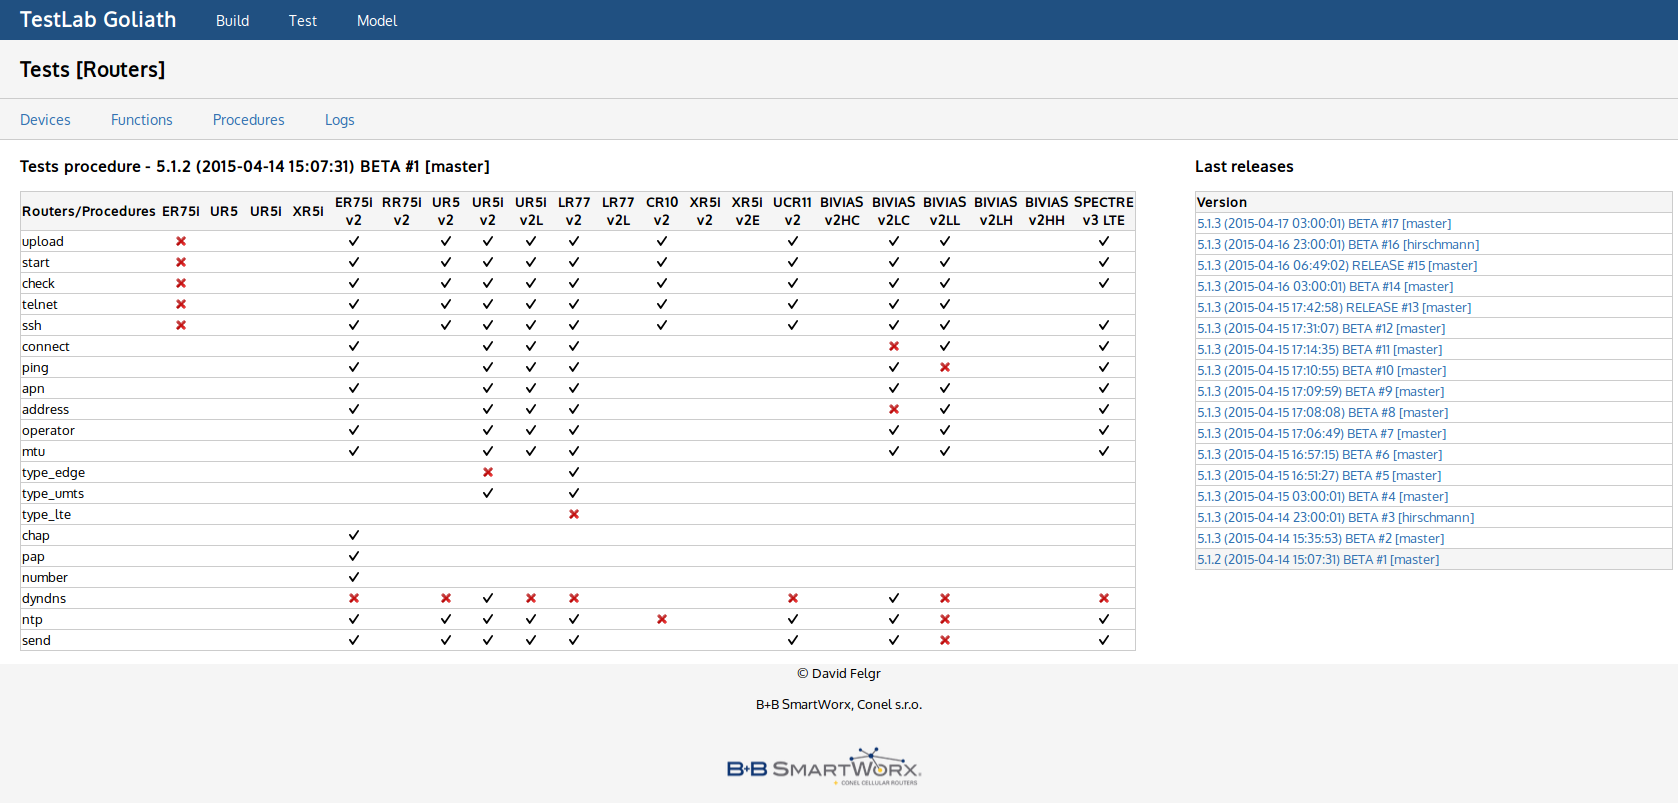
\includegraphics[width=\LW]{web_test_procedure}
  \caption{Stránka product sekce build}
  \label{fig:web_test_device}
\end{figure}

\subsection{Stránka Logs}
Stránka logs je prozatím poslední stránkou sekce test. Na~této stránce jsou zobrazeny všechny chybové hlášky z testovacích procedur. Stránka obsahuje pouze jednu tabulku, kde každý řádek odpovídá jedné chybové hlášce. Tabulka obsahuje celkem pět sloupců. V~prvním sloupci release je zobrazen k jaké testované verzi firmwaru chybová hláška odpovídá. Sloupec router určuje testované zařízení, kde chyba vznikla. Místo, z kterého chybová hláška vzešla, určují následující sloupce function a~procedure. Poslední sloupec event obsahuje samotnou hlášku předanou chybovým výstupem z testovací procedury.

\begin{figure}[h]
  \centering
  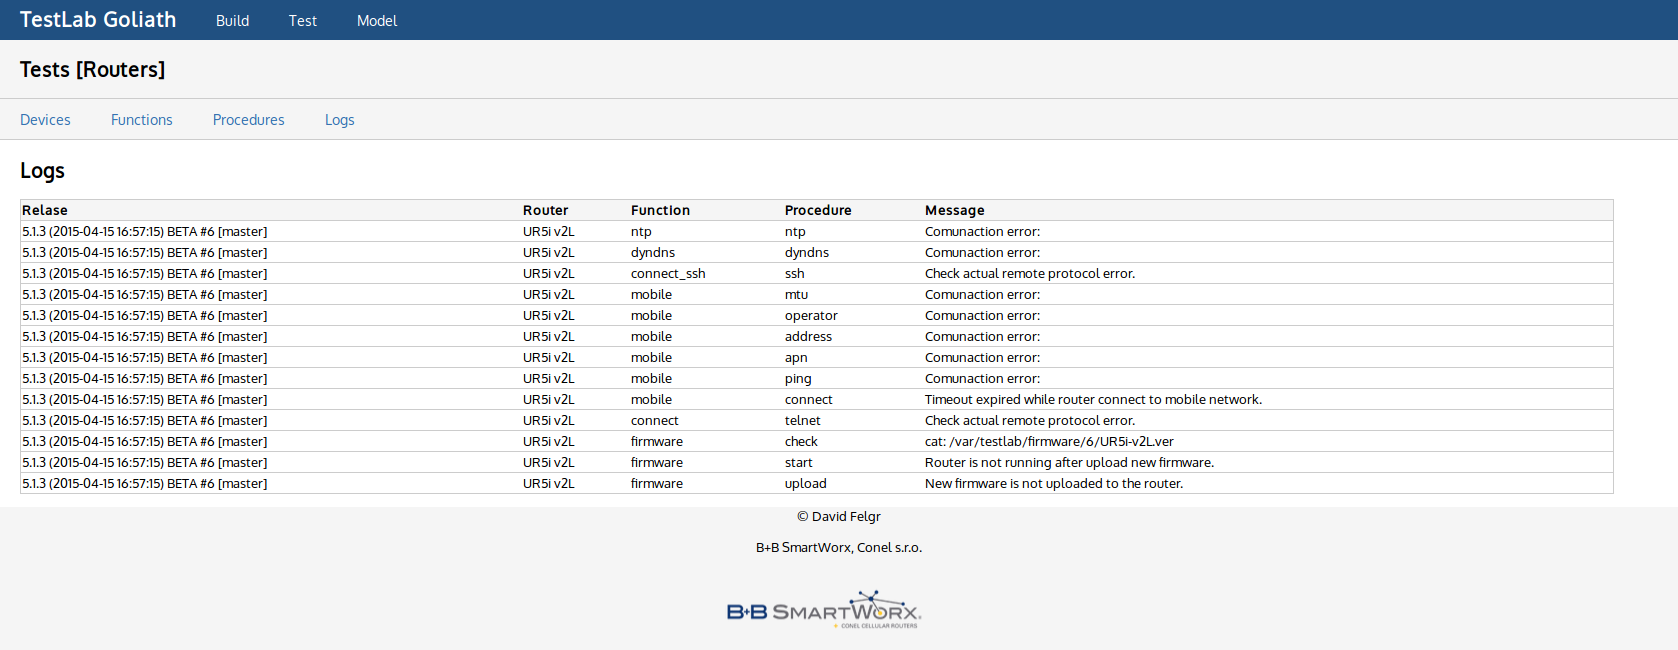
\includegraphics[width=\LW]{web_test_log}
  \caption{Stránka product sekce build}
  \label{fig:web_test_device}
\end{figure}

\endinput
